\chapter{Svolgimento dello \textit{stage}}

\section{Metodo di lavoro}

In questa sezione viene descritto l'approccio organizzativo adottato durante l'intero periodo di \textit{stage}, con particolare attenzione alle modalità di pianificazione delle attività, alla comunicazione con il \textit{tutor} aziendale e agli strumenti utilizzati per monitorare l'avanzamento del progetto.

\subsection{Pianificazione e interazione con il \textit{tutor}}
\label{sec:pianificazione}

%Descrizione dell'organizzazione delle giornate e delle settimane lavorative, della frequenza e delle modalità degli incontri con il \textit{tutor} aziendale, delle revisioni periodiche dello stato di avanzamento e della collaborazione quotidiana con il secondo stagista. Verrà inoltre illustrato l'utilizzo del \textit{file} condiviso \textit{Todo}, impiegato come strumento informale ma efficace per il monitoraggio delle attività aperte e completate, evidenziandone i vantaggi in termini di praticità e i limiti rispetto a sistemi di tracciamento più strutturati.

La Figura~\ref{fig:pianificazione-tutor} offre una visione d'insieme del flusso di pianificazione, interazione con il \textit{tutor} e utilizzo del \textit{file} Todo descritto nel seguito di questa sezione, dalla pianificazione mensile fino al coinvolgimento delle figure di livello superiore verso la fine dello \textit{stage}.
 
\begin{figure}[h]
\centering
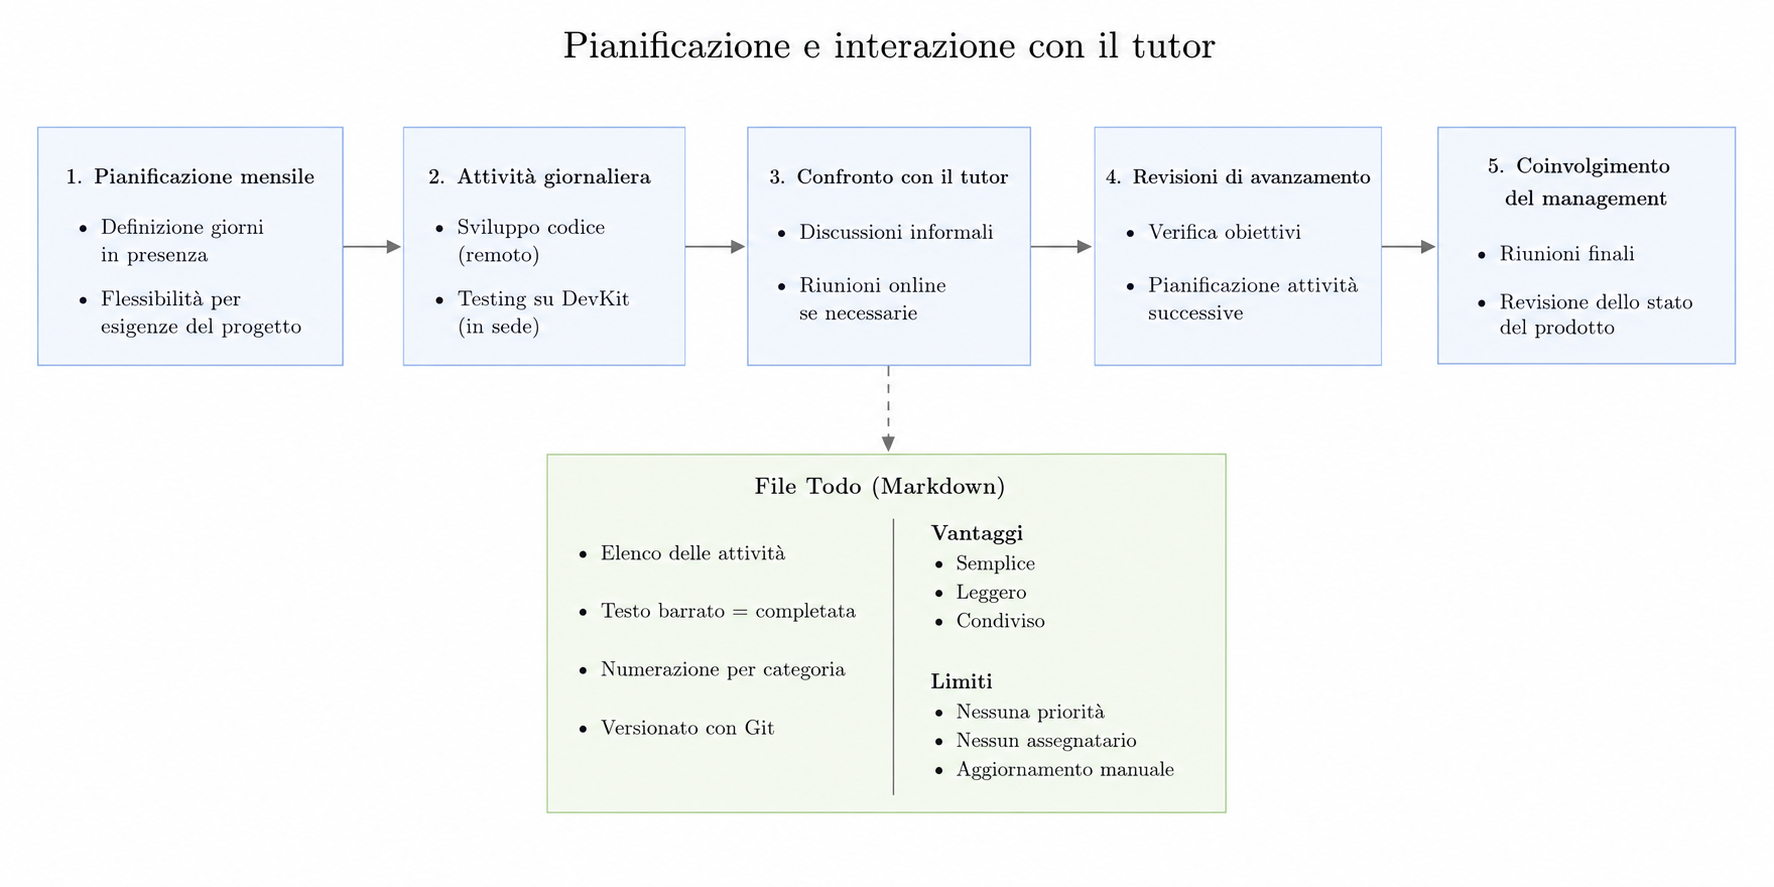
\includegraphics[width=0.95\textwidth]{img/pianificazione_e_interazione.png}
\caption{Flusso di pianificazione mensile, interazione con il \textit{tutor} e utilizzo del \textit{file} Todo}
\label{fig:pianificazione-tutor}
\end{figure}

La pianificazione aziendale prevedeva, come prima cosa di ogni mese, la definizione dei giorni in cui stagisti e dipendenti sarebbero stati in presenza. Questo era dovuto a una scarsità di postazioni di lavoro in grado di accogliere tutti i dipendenti, con l'unica eccezione del venerdì, giorno in cui la maggior parte dei dipendenti lavorava da remoto e restava quindi maggiore flessibilità per noi stagisti. Nel primo mese, maggio, ho lavorato in presenza il martedì e il giovedì; 
nel mese successivo i giorni sono cambiati in lunedì e mercoledì. L'azienda permetteva comunque flessibilità quando il progetto lo richiedeva: nel secondo mese, ad esempio, io e il mio collega stagista siamo andati in azienda con maggiore frequenza, poiché il \textit{Dev Kit} Nintendo Switch necessario per i \textit{test} di certificazione (\ref{sec:obiettivi-controller-certificazione}) era disponibile solo in sede. Nei giorni in cui restavamo a casa, ci concentravamo maggiormente sulla scrittura del codice e meno sulle attività di \textit{\textit{test}ing}, che richiedevano l'accesso diretto alla \textit{console}.
 
La scelta di avere due giorni fissi in presenza faceva parte della strategia con cui comunicavamo con il \textit{tutor}, discutendo gli obiettivi conclusi e quelli futuri. Non esisteva una cadenza fissa di revisione: svolgevamo la maggior parte delle discussioni informalmente in presenza, alla mia postazione o a quella del secondo stagista, ogni volta che vi erano aggiornamenti da condividere. In caso di dubbi sull'avanzamento mentre lavoravamo da remoto, avevamo comunque la possibilità di organizzare riunioni online. Verso la parte finale dello \textit{stage}, quando il gioco assumeva una forma più definita, abbiamo iniziato a organizzare anche alcune riunioni in presenza con figure di livello superiore al nostro \textit{tutor}, responsabili della direzione del prodotto.
 
Nella collaborazione quotidiana con il secondo stagista, abbiamo suddiviso il lavoro per scena piuttosto che per tipo di attività: ciascuno di noi seguiva l'implementazione della navigazione da \textit{controller} su un sottoinsieme di scene, per evitare di lavorare sugli stessi \textit{file} e ridurre il rischio di conflitti in fase di \textit{merge}. Prima di ogni \textit{commit} su una scena condivisa, ci scambiavamo una revisione rapida del codice, più per allineare stile e struttura delle modifiche che come controllo formale di qualità.
 
In modo indipendente dal \textit{tutor}, ma insieme al secondo stagista, abbiamo deciso di non usare uno strumento di tracciamento delle \textit{task} professionale, come quello offerto da GitHub. Abbiamo invece optato per una soluzione meno strutturata, che si è rivelata comunque utile vista la scala ridotta del team.
 
Abbiamo scelto di usare un \textit{file} in formato \textit{markdown}, dove elencavamo tutti gli obiettivi e i problemi che sorgevano man mano e dovevano essere risolti. Il formato \textit{markdown} ci permetteva una visualizzazione grafica sufficiente rispetto all'impegno richiesto, che restava minimo: le uniche decorazioni presenti nel \textit{test}o erano il \textit{test}o sbarrato, usato per segnare una \textit{task} come conclusa, e la dimensione del \textit{test}o, che distingueva i titoli dalle voci delle rispettive liste. Abbiamo strutturato il documento a blocchi, in base alla natura o alla complessità del compito: uno di questi blocchi, ad esempio, teneva traccia dell'implementazione della navigazione da \textit{controller} nelle diverse scene. Per riferirci in modo univoco a ciascuna voce, abbiamo infine introdotto un sistema di numerazione dettato da una lettera, che indicava la categoria, e da un numero, che identificava la voce specifica all'interno della lista.
 
Abbiamo versionato questo documento sin dalla sua creazione, aggiornandolo a ogni \textit{commit} in modo che entrambi potessimo avere sempre la versione più aggiornata sull'avanzamento del progetto.
 
Questa soluzione presentava dei limiti evidenti rispetto a uno strumento di tracciamento professionale: non permetteva di assegnare priorità o scadenze alle singole voci, non offriva visibilità su chi stesse lavorando a una determinata attività in un dato momento, e affidava interamente alla disciplina dei due stagisti la coerenza tra lo stato del \textit{file} e lo stato reale del codice. Con un team di due persone e un ambito di lavoro ben definito, questi limiti non hanno mai causato problemi concreti; la stessa soluzione sarebbe stata probabilmente inadeguata con un team più numeroso o con attività meno prevedibili.
 
\subsection{Versionamento e \textit{workflow} collaborativo}

% Descrizione dell'utilizzo di \textit{Git} e \textit{Bitbucket} per la gestione del codice sorgente, dell'organizzazione dei rami di sviluppo, delle operazioni di \textit{merge} tra il lavoro dei due stagisti e delle modalità di rilascio progressivo delle modifiche. Verrà inoltre evidenziato come la struttura dei messaggi di \textit{commit} abbia costituito una forma di documentazione incrementale dell'evoluzione del progetto, compensando l'assenza di un sistema dedicato di \textit{issue tracking}.

Per il versionamento del progetto, come già accennato nel primo capitolo, abbiamo usato il software Git insieme a Bitbucket, ospitato su un'infrastruttura indipendente dall'azienda.
 
Quando ho preso in mano il progetto, l'organizzazione dei rami era piuttosto caotica: erano aperti numerosi \textit{branch}, conseguenza diretta dell'assenza di manutenzione del progetto negli anni precedenti allo \textit{stage}. Molti di questi rami avevano nomi poco significativi, riferiti solamente alle persone che vi avevano lavorato in passato.
 
Per lo \textit{stage}, insieme al \textit{tutor} abbiamo deciso di creare un nuovo \textit{branch} a partire dall'ultimo \textit{commit} disponibile, risalente al 2018. Nelle prime due settimane, in cui ero l'unico stagista sul progetto, ho lavorato direttamente su questo \textit{branch}, senza dover gestire conflitti di \textit{merge}. Quando è arrivato il secondo stagista, abbiamo invece scelto di creare due rami separati: uno dedicato ai miei compiti, l'altro ai suoi.
 
%\textbf{\{DA COMPLETARE: come avvenivano concretamente i merge tra i due \textit{branch}? Pull request su Bitbucket con revisione incrociata, merge diretto da riga di comando, altro?\}}
 
La collaborazione tra i due \textit{branch} si basava su una regola semplice: comunicare preventivamente su quali scene o \textit{file} ciascuno stesse lavorando, per poi dividersi le \textit{task} di conseguenza ed evitare di modificare gli stessi \textit{file} in parallelo. Prima di integrare il proprio lavoro nel \textit{branch} principale creato a inizio \textit{stage}, verificavamo che le modifiche non introducessero errori nel codice.
 
%\textbf{\{DA COMPLETARE: come arrivava il codice dai \textit{branch} di lavoro a una build effettivamente distribuita o \textit{test}abile? C'era una cadenza di rilascio, un \textit{branch} di destinazione comune, dei tag di versione?\}}
 
Le descrizioni dei messaggi di \textit{commit} costituivano inoltre una forma di documentazione incrementale del progetto, che compensava l'assenza di uno strumento dedicato di \textit{issue tracking} descritta in \ref{sec:pianificazione}. Per riferirci in modo univoco alle voci del \textit{file} Todo presentato in quella stessa sezione, anteponevamo ai messaggi di \textit{commit} la sigla \texttt{td}, seguita dalla lettera della categoria e dal numero della voce specifica: un \textit{commit} relativo, ad esempio, alla voce C3 del \textit{file} Todo riportava la dicitura \texttt{td-C3}. Questa convenzione ci permetteva di ricostruire, a posteriori, quale attività pianificata ciascuna modifica al codice avesse implementato.

\section{Attività svolte}

Presento le attività sviluppate nel corso delle otto settimane di \textit{stage} secondo una suddivisione per macroaree di progetto, anziché seguire una successione cronologica. Per ciascuna attività, descrivo il requisito da soddisfare, le scelte progettuali adottate, la relativa implementazione e le modalità con cui ne ho verificato la correttezza.

\subsection{Stabilizzazione del progetto su Unity 6}
\label{sec:migrazione-progetto}

%Il lavoro iniziale dello stage è stato dedicato all'aggiornamento dell'ambiente di sviluppo mediante la migrazione del progetto a \textit{Unity 6}. In questo contesto sono stati individuati e risolti numerosi problemi di compatibilità, tra cui errori di rendering delle immagini dovuti all'inversione dell'ordine di visualizzazione e malfunzionamenti delle \textit{shader} causati dal nuovo motore grafico. Verrà descritto il processo di analisi adottato per individuare le cause dei problemi e le soluzioni implementate, con particolare attenzione agli aspetti tecnici che hanno contribuito maggiormente alla crescita professionale maturata durante lo stage.
 
L'obiettivo di questa attività, completata nelle prime due settimane di \textit{stage}, era migrare il progetto da Unity 2017 a Unity 6 senza errori di compilazione, come definito in \S\ref{sec:obiettivi-migrazione-engine}. Il progetto presentava un salto di sei versioni principali dell'engine, con potenziali incompatibilità distribuite su motore grafico, sistema di \textit{input}, librerie di terze parti e configurazione di \textit{build} per ciascuna piattaforma.
 
Per affrontare questo aggiornamento, ho scelto di dividerlo in due passaggi, inserendo una versione intermedia tra quella di partenza e quella finale, anziché saltare direttamente da Unity 2017 a Unity 6. Questa scelta riduceva il rischio di perdere traccia di errori che, saltando subito a una versione molto più recente, l'engine potrebbe non segnalare più affatto: il codice ormai troppo datato viene infatti rimosso dalle versioni più recenti, anziché semplicemente segnalato come deprecato. La versione scelta come tappa intermedia è stata Unity 2021, un compromesso tra la versione di partenza (rilasciata nel 2017) e la versione 6, obiettivo finale, rilasciata nel 2025. La Figura~\ref{fig:line-versioni-unity} riassume questo percorso a tappe.
 
\begin{figure}[H]
    \centering
    \makebox[\textwidth][c]{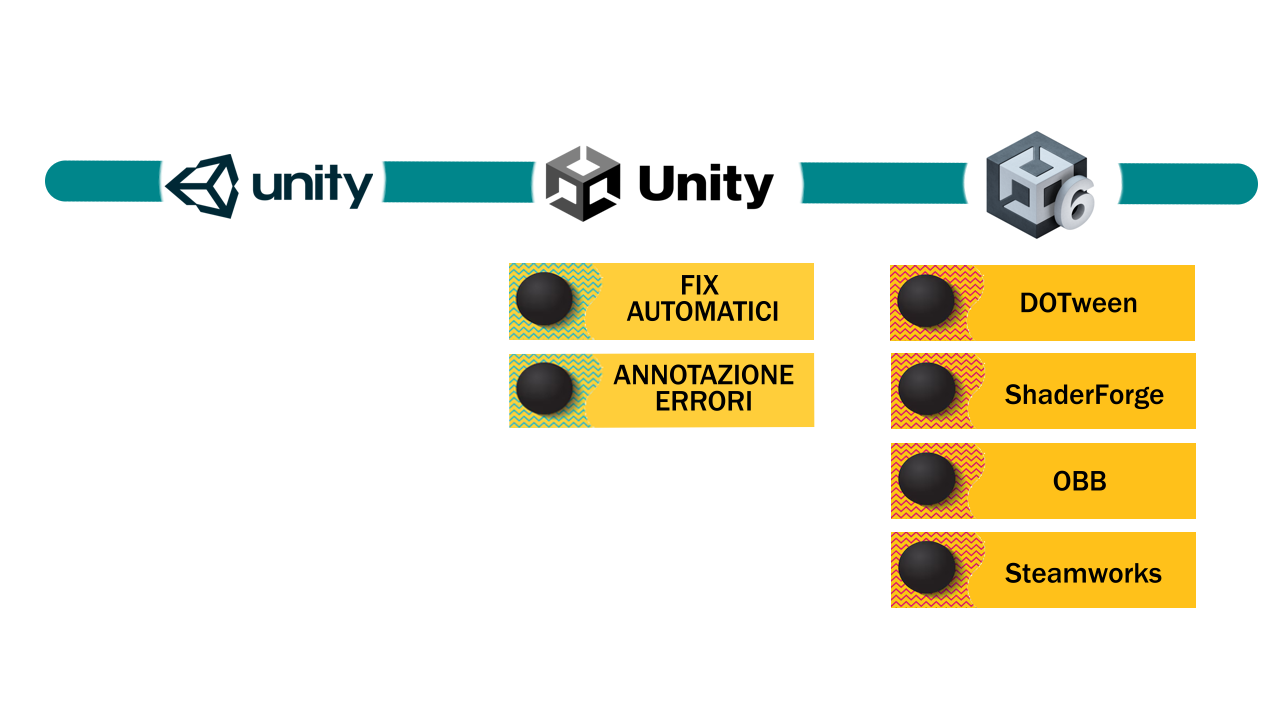
\includegraphics[width=1.15\textwidth]{img/linea_versioni_unity.png}}
    \caption{Grafico riassuntivo delle migrazioni effettuate}
    \label{fig:line-versioni-unity}
\end{figure}
 
Il primo passaggio, da Unity 2017 a Unity 2021, è stato in gran parte gestito dall'engine stesso: Unity individuava automaticamente le impostazioni non più compatibili e proponeva direttamente la correzione da applicare. Un esempio è l'impostazione \textit{Auto Graphics API}, che Unity segnalava come da aggiornare per allinearsi alle API grafiche supportate dalle versioni più recenti dell'engine; ho applicato la correzione seguendo l'indicazione proposta nei \textit{settings} del progetto. In questa tappa mi sono limitato ad annotare gli errori più complessi emersi in console, rimandandone la risoluzione al passaggio successivo, senza intervenire direttamente nel codice.
 
Il secondo passaggio, da Unity 2021 a Unity 6, ha richiesto interventi più sostanziali. Alcune dipendenze sono state aggiornate automaticamente dall'engine, senza richiedere intervento diretto: \textit{DOTween}, una libreria molto diffusa nell'ecosistema Unity per la gestione semplificata della fisica 2D, rientra in questo caso, poiché il progetto la includeva come file \texttt{.dll} (una libreria già compilata) anziché come pacchetto Unity, e l'engine la riconosceva quindi automaticamente attraverso il \textit{Package Manager}.
 
Per la libreria \textit{ShaderForge}, invece, non emergevano errori espliciti di compilazione, né inizialmente problemi visibili all'interno del gioco: gli errori comparivano solo selezionando una \textit{shader} creata tramite l'interfaccia grafica offerta dalla libreria, a causa della mancanza di alcuni pulsanti nella finestra \textit{Inspector}. Testando il gioco nell'\textit{editor} nel corso delle settimane, io e il mio collega abbiamo notato alcuni artefatti grafici non coerenti con la versione rilasciata su Steam nel 2018, riguardanti principalmente la trasparenza di alcune texture. Le soluzioni possibili erano due: ricreare da zero le \textit{shader} problematiche tramite l'interfaccia grafica di ShaderForge, oppure intervenire direttamente sul codice generato — tecnica più scomoda, dato che di norma le shader si costruiscono tramite strumenti grafici dedicati. Ho scelto la seconda opzione nonostante la maggiore difficoltà, per ragioni di tempo. Il problema principale risiedeva in una proprietà di \textit{blend} alpha non più configurata correttamente, responsabile della trasparenza rotta osservata sulle texture; ho inoltre corretto alcuni valori di colore che, pur non generando errori, risultavano visibilmente diversi dalla versione rilasciata su Steam nel 2018. Non disponendo dei valori originali, li ho regolati per confronto visivo diretto con la \textit{build} di riferimento, facendoli approvare dal tutor una volta completato il lavoro.
 
Una serie di \textit{warning} riguardava inoltre il rimpiazzo di alcuni metodi ormai obsoleti, ripetuti in diverse parti del codice del gioco: l'avanzamento delle versioni di Unity aveva infatti deprecato questi metodi. La sostituzione è stata comunque semplice, poiché l'engine indicava già, all'interno del \textit{warning} stesso, la nuova firma del metodo da utilizzare; ho dovuto soltanto adattare i parametri passati, senza altre modifiche.
 
Un problema distinto riguardava la \textit{build} Android, alle prese con l'uso degli \textit{OBB}: sebbene i file OBB restino tecnicamente utilizzabili nell'ecosistema Android, non sono più ammessi per la pubblicazione sul Google Play Store, e la libreria \textit{OBB Downloader}, ancora presente nel progetto, generava quindi errori. È bastato rimuovere la cartella che la conteneva per eliminarli.
 
L'interazione con Steam era invece affidata alla libreria \textit{Steamworks.NET}, che il progetto originale includeva scaricando i file binari e importandoli direttamente, senza passare dal \textit{Package Manager} — una scelta dovuta al fatto che la libreria non era ufficialmente supportata da Unity al momento della sua integrazione originaria, a differenza delle versioni più recenti dell'engine, che supportano anche librerie non ufficiali e provenienti da fonti diverse dallo \textit{store}. Ho risolto il problema eliminando completamente la cartella esistente e importando la versione più recente della libreria tramite il \textit{Package Manager}. Questa correzione ha però introdotto un nuovo problema: una volta caricata correttamente, la libreria rendeva il gioco impossibile da eseguire dall'\textit{editor}, poiché, per costruzione, apriva il client Steam per avviare il gioco dalla collezione giochi dell'\textit{account}, eseguendo di conseguenza la versione rilasciata nel 2018 anziché quella in sviluppo. Per aggirare questo problema, abbiamo utilizzato le direttive di compilazione condizionale di Unity (\texttt{\#if UNITY\_EDITOR}), escludendo l'inizializzazione della libreria dalle \textit{build} generate per l'\textit{editor}: in questo modo il codice di avvio di Steamworks non viene proprio incluso in quella configurazione, anziché essere semplicemente ignorato a \textit{runtime}. \textbf{\{DA COMPLETARE: ruolo esatto del simbolo DISABLESTEAMWORK e come si relaziona a questa direttiva — in attesa dello snippet di codice.\}}
 
Infine, un ultimo gruppo di problemi riguardava elementi grafici — testi e immagini dinamiche — localizzati nella scena \textit{Dungeon Game}. Al primo accesso, una schermata con una \textit{texture} di legno occupava l'intero campo visivo dell'utente; dopo tre \textit{click} a vuoto, l'immagine si nascondeva e si poteva procedere senza problemi. Questo artefatto, apparentemente incomprensibile, non era altro che un \textit{tutorial} composto da tre immagini che scorrevano al \textit{click} del \textit{mouse}, ma che restavano nascoste dietro al proprio sfondo. Un problema della stessa natura si presentava una volta sconfitta una stanza, quando le descrizioni previste sotto le immagini di un forziere e di un portale non comparivano, lasciando visibile solo il loro sfondo. Abbiamo attribuito entrambi i problemi al cambio nella gestione del \textit{rendering} degli oggetti di scena introdotto da Unity: senza l'intervento del codice, che può attivare o disattivare gli oggetti nella scena, il motore grafico disegna a schermo tutti gli oggetti nell'ordine in cui compaiono nella gerarchia della scena. Abbiamo risolto il problema riordinando manualmente gli sfondi delle immagini e dei testi problematici più in alto nella \textit{Hierarchy} della scena, in modo che il motore li disegnasse per primi. Il primo tentativo, effettuato spostando gli oggetti direttamente durante l'esecuzione del gioco nell'\textit{editor}, non produceva un cambiamento persistente: Unity non salva le modifiche apportate alla gerarchia in modalità \textit{Play}. Abbiamo quindi ripetuto lo stesso riordinamento a gioco fermo, direttamente sugli \textit{asset} della scena.
 
Una volta stabilizzate le \textit{build}, ovvero eliminati gli errori di compilazione, la verifica si è concentrata sul controllo quotidiano che le modifiche apportate funzionassero correttamente non solo nell'\textit{editor}, ma anche nel reale ambiente di esecuzione di ciascuna piattaforma, poiché alcuni errori non risultano simulabili all'interno dell'ambiente di sviluppo. Il PC è risultato la piattaforma meno problematica, sia perché il primo sviluppo del gioco era stato realizzato per questa piattaforma, sia perché testare da \textit{computer} non richiede l'installazione dell'applicazione né il trasferimento di file su un dispositivo esterno. Anche il \textit{mobile} è stato semplice da verificare: la maggior parte dei problemi residui riguardava le \textit{shader}, dovuti alle diverse \textit{API} native del dispositivo. L'ecosistema Apple ha richiesto un approccio diverso: pur avendo sviluppato e testato fin dall'inizio in ambiente Windows, eseguire il gioco su un Mac o un iPhone richiede necessariamente un dispositivo Apple su cui aprire il progetto ed eseguire le \textit{build}. Abbiamo quindi svolto tutte le prove per questo ecosistema alla fine dello sviluppo, quando sapevamo che non avremmo più toccato nulla che potesse comprometterlo; a parte questo rallentamento e un piccolo problema grafico dovuto a una scelta di programmazione del team di sviluppo precedente, l'ambiente Apple non ha dato ulteriori problemi.
 
Proprio per verificare in modo efficace gli errori non riproducibili nell'\textit{editor}, abbiamo deciso di creare un \textit{logger}: una semplice interfaccia grafica che stampava a schermo qualunque comunicazione il gioco avrebbe dovuto stampare — \textit{warning}, errori, oppure \textit{print} inseriti esplicitamente nel codice da me e dal mio collega, o già presenti nella vecchia versione del gioco (Figura~\ref{fig:unity-logger-game}). Questo strumento non sarebbe stato necessario testando solo all'interno di Unity, che offre una \textit{console} di \textit{debug} che svolge lo stesso lavoro; per le applicazioni eseguite nel loro reale ambiente di esecuzione, invece, questo approccio si è rivelato molto più veloce da implementare e immediato nella verifica rispetto a \textit{software} di terze parti, a patto di ricordarsi di disabilitarlo al momento del rilascio sulle piattaforme ufficiali.
 
\begin{figure}[H]
    \centering
    \makebox[\textwidth][c]{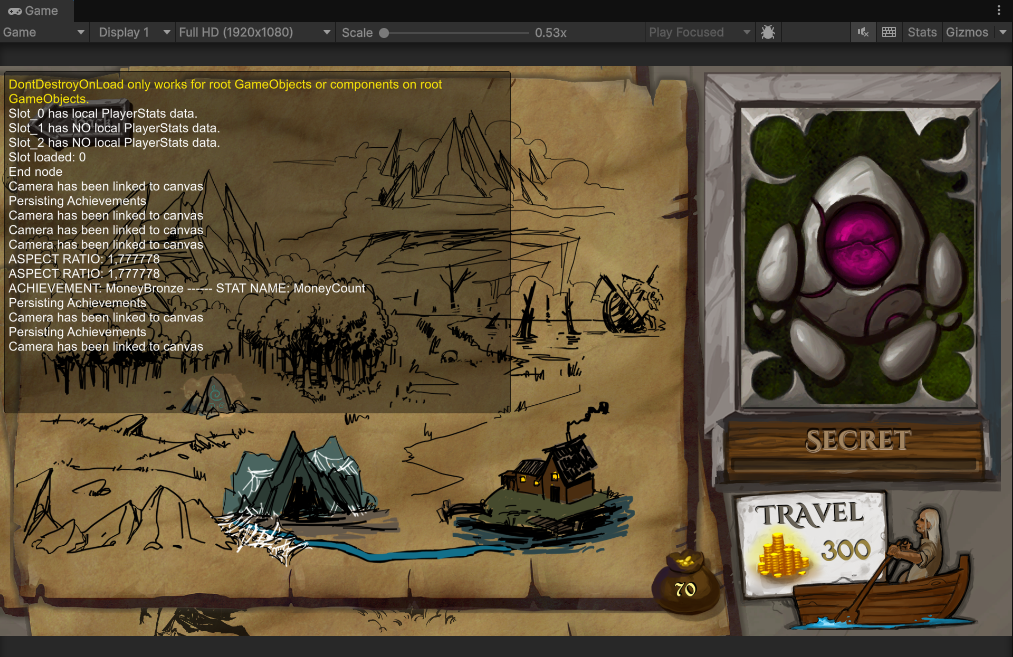
\includegraphics[width=1.15\textwidth]{img/unity_logger_game.png}}
    \caption{Interfaccia del \textit{logger} all'interno del gioco}
    \label{fig:unity-logger-game}
\end{figure}

\subsection{Implementazione della navigazione da \textit{controller}}
\label{sec:implementazione_controller}
 
%L'attività principale dello stage ha riguardato la progettazione e l'implementazione della navigazione completa tramite gamepad, inizialmente sviluppata utilizzando un controller PlayStation 4, su tutte le scene del gioco: Authentication, Inn, Dungeon Choose, DeckBuilder, InventoryShop e DungeonGame. Verranno illustrate le principali sfide affrontate durante lo sviluppo, tra cui la progettazione di una logica unificata per la funzione Back, l'introduzione dei pulsanti L1 e R1 nella schermata DeckBuilder, la realizzazione del cursore grafico a forma di mano per evidenziare il \textit{focus} corrente e le strategie adottate per adattare al controller un'interfaccia originariamente progettata per dispositivi mouse e touch.
 
L'obiettivo di questa attività era realizzare una navigazione completa tramite \textit{gamepad} su tutte e sei le scene del gioco, come definito in \S\ref{sec:obiettivi-controller-certificazione}. Il progetto, sviluppato originariamente per \textit{PC}, offriva un'interfaccia pensata esclusivamente per \textit{mouse} e tastiera: analizzando il sistema di \textit{input} allora in uso in Unity — il Legacy Input Manager, basato sulla lettura diretta dello stato delle periferiche tramite le API di \textit{input} — sono emersi diversi limiti nel momento in cui si è reso necessario estendere il supporto ai \textit{controller}, poiché ogni nuova periferica richiede generalmente l'aggiunta o la modifica delle mappature di \textit{input} esistenti. Per lo sviluppo e i primi \textit{test} ho utilizzato un \textit{controller} \textit{PlayStation 4}, poiché era quello già disponibile in azienda; una volta avviati i \textit{test} sulla \textit{build} per Nintendo Switch, abbiamo esteso il supporto ai \textit{controller} nativi della \textit{console} — Joy-Con e Pro Controller.
 
La migrazione del progetto a Unity 6 (\S\ref{sec:migrazione-progetto}) ha rappresentato l'occasione per adottare il New Input System, distribuito come \textit{package} ufficiale di Unity: la sua adozione non è stata una semplice sostituzione delle \textit{API} esistenti, ma un requisito fondamentale per la realizzazione della navigazione tramite \textit{gamepad}. A differenza del Legacy Input Manager, questo sistema non si basa esclusivamente sulla lettura dello stato dei dispositivi, ma introduce un livello di astrazione fondato sul concetto di Input Action: lo sviluppatore non associa più direttamente una funzione a uno specifico tasto, bensì definisce un'azione logica — come \textit{Navigate}, \textit{Submit} o \textit{Cancel} — alla quale è possibile collegare più dispositivi e più controlli contemporaneamente (Figura~\ref{fig:confronto-input-systems}). Questa astrazione consente di separare la logica dell'applicazione dalla periferica utilizzata, permettendo di gestire tastiera, \textit{mouse}, \textit{gamepad} e dispositivi \textit{touch} attraverso lo stesso insieme di azioni: è lo stesso principio che ha poi permesso di estendere il supporto ai \textit{controller} nativi Switch semplicemente aggiungendo i comandi corrispondenti alle Input Action già definite, senza modificare la logica di navigazione sottostante.
 
\begin{figure}[H]
    \centering
    \makebox[\textwidth][c]{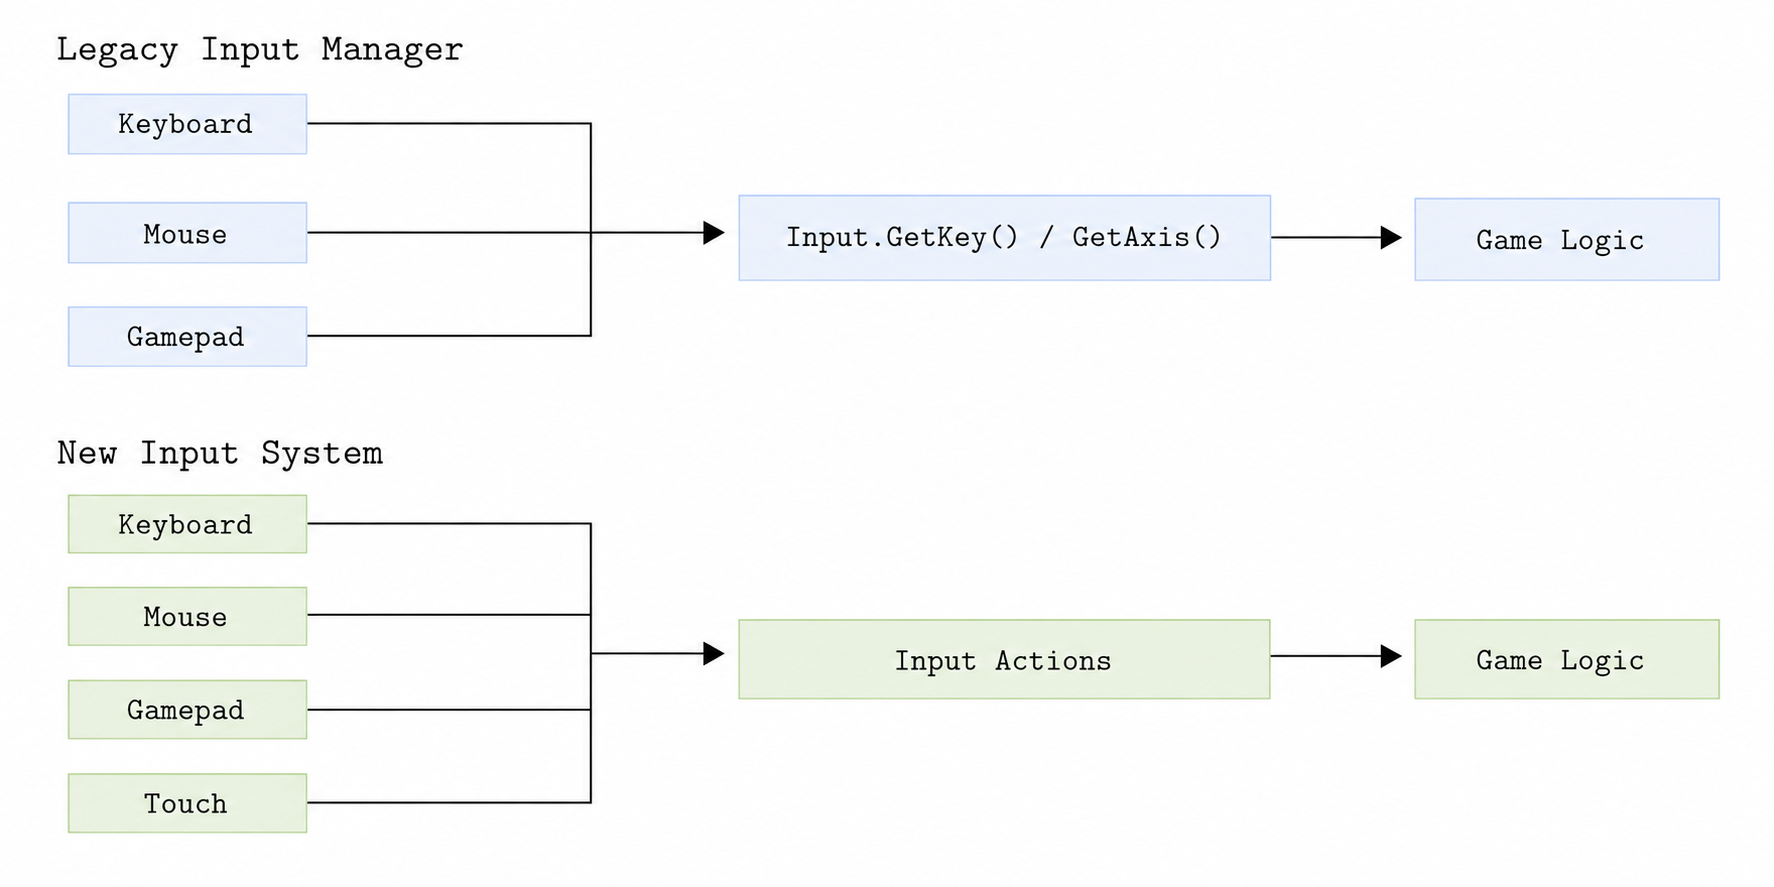
\includegraphics[width=1.15\textwidth]{img/confronto_input.png}}
    \caption{Confronto schematico tra i due sistemi di \textit{input} in Unity}
    \label{fig:confronto-input-systems}
\end{figure}
 
Poiché l'interfaccia originale era stata progettata esclusivamente per \textit{mouse} e dispositivi \textit{touch}, la scelta progettuale centrale è stata definire un modello di navigazione che permettesse di raggiungere qualsiasi elemento interattivo esclusivamente mediante il \textit{gamepad}. Il New Input System offre a questo scopo la possibilità di collegare tra loro gli elementi selezionabili dell'interfaccia lungo le quattro direzioni cardinali — uno strumento pensato per muoversi in un menu, o in un gioco 2D come questo, senza il supporto di un cursore. Il collegamento generato automaticamente dal sistema, tuttavia, si limita a collegare a ogni pulsante i quattro oggetti più vicini nelle diverse direzioni, senza tenere conto della logica di interfaccia né di quando un elemento risulti effettivamente attivo: la scelta progettuale conseguente è stata quindi configurare manualmente, scena per scena, i collegamenti direzionali corretti, evitando che pulsanti mai visibili contemporaneamente sullo schermo risultassero collegati tra loro.
 
A partire da questa base, abbiamo definito alcune regole di progettazione comuni a tutte le scene: gli elementi con un'unica interazione possibile e priva di effetti collaterali immediati — come gli slot di salvataggio, le classi del personaggio o le carte nel Deck Builder — vengono selezionati automaticamente non appena ricevono il \textit{focus}, riducendo il numero di pressioni necessarie per le operazioni più frequenti. Per le funzionalità secondarie o poco frequenti, come l'accesso ai crediti o il cambio di categoria nel Deck Builder, abbiamo scelto di isolarle dal grafo di navigazione principale tramite tasti dedicati (rispettivamente Y/Triangle e L1/R1), anziché complicare i collegamenti tra gli elementi usati più di frequente.
 
Un'ulteriore scelta progettuale ha riguardato l'unificazione della logica del tasto \textit{Back} con l'\textit{Escape Logic} già presente nel progetto — uno script scritto dagli sviluppatori originali per gestire il ritorno alla scena \textit{Inn} da qualunque altra scena, collegato anche al tasto \texttt{Esc} come scorciatoia. Una singola pressione rischiava di attivare contemporaneamente entrambe le logiche: la soluzione progettuale è stata introdurre, nelle scene interessate, eventi attivati ogni volta che appariva un nuovo menu, in grado di aggiornare dinamicamente quale delle due logiche dovesse gestire l'azione in base alla presenza o meno di un sottomenu aperto.
 
Infine, la gestione del \textit{focus} — l'elemento dell'interfaccia che riceve gli \textit{input} del \textit{controller} in un dato istante — ha richiesto una strategia dedicata per il recupero automatico del \textit{focus} corretto quando il giocatore passava dal \textit{mouse} al \textit{gamepad}, evitando che la navigazione ripartisse da elementi arbitrari o non più visibili. Per rendere questo stato sempre riconoscibile, abbiamo scelto di introdurre un cursore grafico a forma di mano, dopo che una prima soluzione basata sulla sola variazione cromatica dell'elemento selezionato si era rivelata non sempre sufficientemente evidente.
 
L'introduzione del New Input System nel progetto è avvenuta in modo progressivo: nelle impostazioni di Unity abbiamo mantenuto l'opzione Input System Package (New) + Input Manager (Old), corrispondente alla modalità Both, che consentiva al codice esistente di continuare a utilizzare il Legacy Input Manager mentre sviluppavamo le nuove funzionalità con il New Input System. Questa soluzione aveva carattere esclusivamente temporaneo, ma si è rivelata fondamentale: ci ha permesso di verificare il corretto funzionamento dell'intero gioco anche quando avevamo già convertito solo alcune scene al nuovo sistema, evitando di dover completare la migrazione prima di poter eseguire \textit{test} significativi.
 
Una volta predisposto l'ambiente di lavoro, abbiamo individuato le funzionalità comuni a tutte le scene e le abbiamo definite come Input Action indipendenti dalla scena corrente — tra le prime, la navigazione tra gli elementi dell'interfaccia, la conferma di una selezione e l'annullamento dell'operazione corrente (Back). Per ciascuna scena abbiamo poi progettato uno schema che definisse esplicitamente le relazioni di adiacenza tra gli elementi selezionabili, facendo attenzione al fatto che una stessa scena potesse gestire più interfacce sovrapposte — ad esempio un sottomenu che compariva dopo aver premuto un determinato pulsante — e modificando singolarmente ogni riferimento di navigazione per riflettere questi collegamenti corretti.
 
La Figura~\ref{fig:schema-navigazione-inn} mostra lo schema di adiacenza implementato per la schermata \textit{Inn}, una delle scene più articolate dal punto di vista della navigazione poiché funge da \textit{hub} verso tutte le altre schermate del gioco (\S\ref{sec:prodotto-litd}) e racchiude contemporaneamente più parti del gioco — il \textit{tutorial}, l'accesso alle altre scene, i crediti.
 
\begin{figure}[H]
    \centering
    \makebox[\textwidth][c]{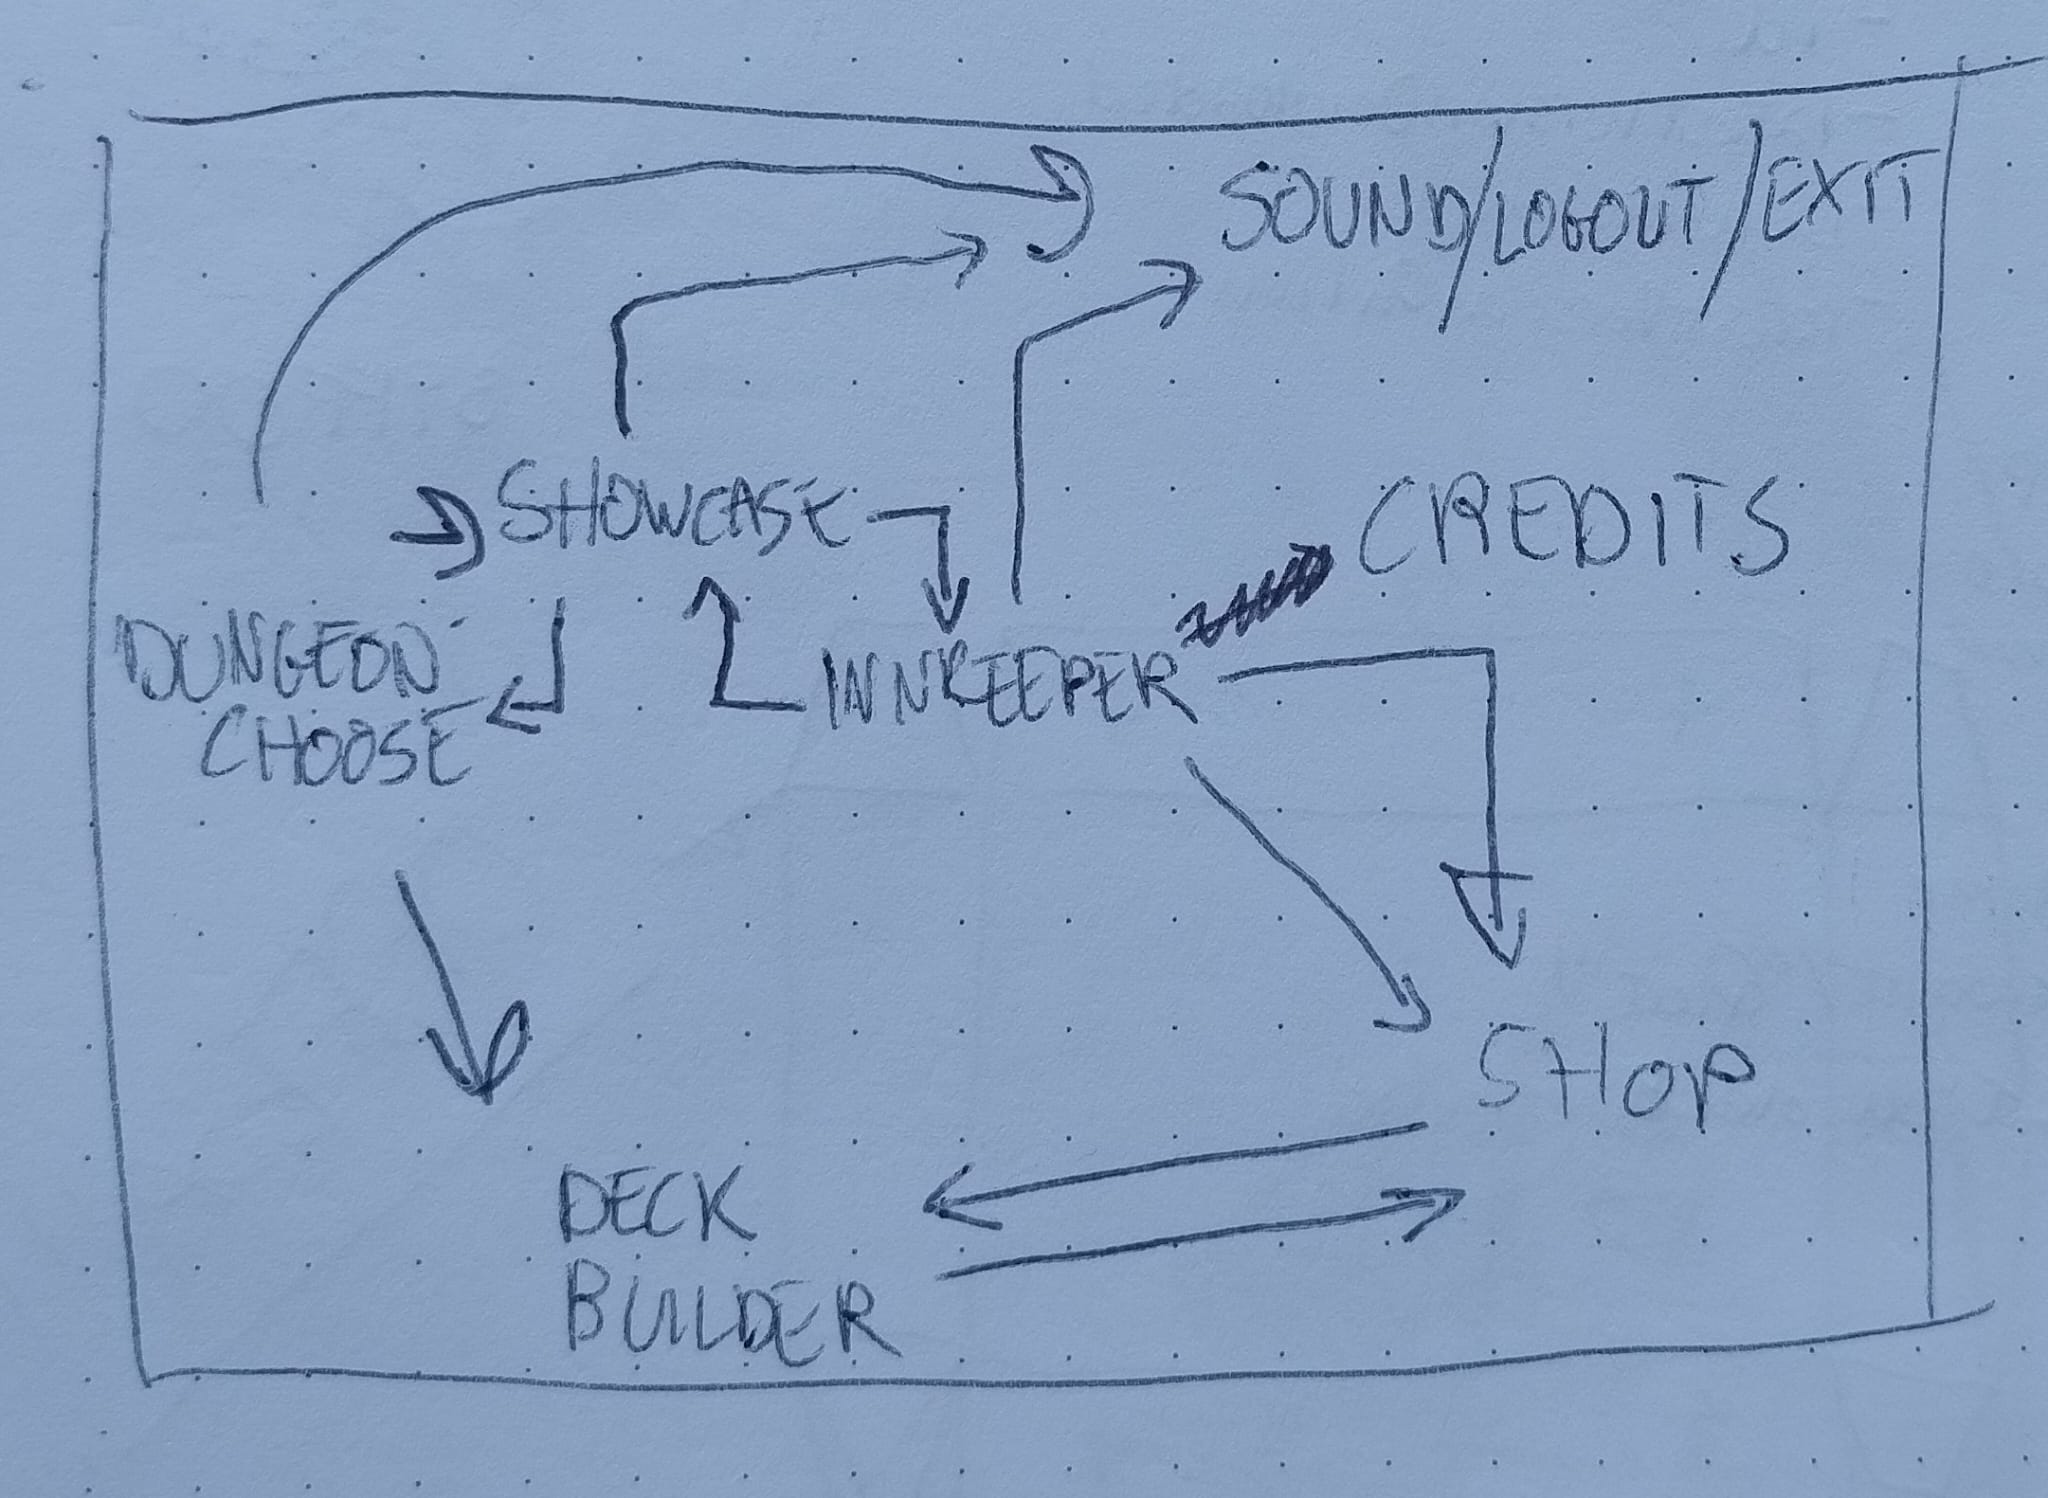
\includegraphics[width=1.15\textwidth]{img/inn_scene_appunti.jpeg}}
    \caption{Schizzo della navigazione \textit{controller} nella scena Inn}
    \label{fig:schema-navigazione-inn}
\end{figure}
 
In \textit{Inn}, coerentemente con la scelta progettuale di isolare le funzionalità secondarie, abbiamo reso la schermata dei crediti raggiungibile solo tramite il tasto dedicato Y/Triangle (da \textit{mouse} resta sufficiente cliccarci sopra). Nella sezione di \textit{tutorial}, invece, abbiamo disabilitato del tutto la navigazione libera: il giocatore può interagire solo con il personaggio del \textit{Ferryman} per accedere al dialogo introduttivo, e in seguito solo con l'elemento che avvia il primo \textit{dungeon} — una sequenza fissa di due soli punti di interazione, pensata per guidare i primi passi senza margine di errore. Questi due casi, insieme all'uso dei tasti L1/R1 nel Deck Builder, mostrano come lo stesso principio progettuale — tasti dedicati per isolare funzionalità secondarie dal flusso di navigazione principale — si ripeta in scene diverse del gioco.
 
Per il conflitto tra \textit{Back} ed \textit{Escape Logic}, l'implementazione ha previsto l'inserimento di eventi, attivati alla comparsa di un nuovo menu, che aggiornano una condizione (\texttt{if}) verificando se il giocatore si trovi ancora all'interno di un sottomenu, decidendo di conseguenza quale delle due logiche debba gestire l'azione.
 
Il cursore a forma di mano, infine, accompagna costantemente il \textit{focus} corrente, rendendo immediatamente riconoscibile l'elemento che riceverà il successivo \textit{input} del giocatore.
 
La modalità Both, oltre a facilitare l'introduzione progressiva del nuovo sistema, ha costituito il principale strumento di verifica di questa attività: ha permesso di testare l'intero gioco in ogni momento della conversione, anziché solo al suo completamento. La verifica definitiva del rispetto del requisito imposto dal \textit{platform holder} — la navigazione tramite \textit{controller} su tutte le scene — è avvenuta nell'ambito del processo di certificazione Nintendo Switch, descritto nella sezione seguente (\S\ref{sec:certificazione-switch}).
 
\subsection{Certificazione Nintendo Switch}
\label{sec:certificazione-switch}

%Particolare attenzione verrà dedicata al processo di certificazione Nintendo Switch, durante il quale è stato individuato il superamento del limite di Write Access Count. Verranno descritte le attività di analisi delle cause, le ottimizzazioni introdotte per ridurre il numero di accessi in scrittura e il successivo superamento del requisito di certificazione.

La certificazione Nintendo Switch imponeva due requisiti principali sul progetto: la navigazione completa tramite \textit{controller}, requisito del \textit{platform holder} già descritto in \S\ref{sec:implementazione_controller} — poiché, sebbene i controlli \textit{touch} siano supportati, il principale strumento con cui i giocatori si interfacciano a ogni gioco resta il \textit{controller} — e la conformità del sistema di salvataggio a sei \textit{test} ufficiali, riassunti in Tabella~\ref{tab:test-nintendo-salvataggi}.

Per quanto riguarda l'\textit{hardware}, inizialmente non sapevamo quanto ci saremmo avvicinati a una versione rilasciabile del gioco: di conseguenza, l'azienda non aveva deciso di investire subito nell'acquisto del \textit{Dev Kit} Nintendo Switch, l'ambiente di sviluppo ufficiale della piattaforma. Per alcune settimane abbiamo quindi provato il gioco usando una Nintendo Switch \textit{moddata}, modificata con un \textit{software} che ne cambia radicalmente il funzionamento, permettendo ad esempio di ricevere \textit{file} dal \textit{computer} e installare \textit{file} \texttt{.nsp}.

Il primo vincolo tecnico incontrato riguardava proprio il sistema di salvataggio: il \textit{file system} della \textit{console} funziona in modo sostanzialmente diverso da quello di un comune \textit{computer}, anche per la natura più chiusa della piattaforma rispetto a un PC. Attraverso la documentazione ufficiale fornita da Nintendo agli sviluppatori, abbiamo capito che serviva configurare un tipo di scrittura e lettura specifico, utilizzando le \textit{API} messe a disposizione dall'\textit{SDK} della \textit{console}: per scrivere qualcosa in memoria è necessario prima instanziare, o selezionare, l'area di \textit{mount}, operazione per cui serve un riferimento allo \textit{userid}. I dati vengono inoltre scritti solo su un \textit{buffer} e non direttamente in memoria: per renderli persistenti è necessario un \textit{commit}, un'operazione che libera il \textit{buffer} scrivendo definitivamente le informazioni al suo interno nelle celle di memoria assegnate.

\begin{table}[h]
\centering
\begin{tabular}{|c|p{10cm}|}
\hline
\textbf{Test} & \textbf{Ambito verificato} \\
\hline
1 & Continuità del salvataggio dopo il trasferimento dei dati tra \textit{account} utente tramite \textit{backup} su scheda SD \\
\hline
2 & Continuità del salvataggio dopo un cambiamento dell'identificativo di sistema \\
\hline
3 & Continuità del salvataggio al variare dell'\textit{account} Nintendo collegato all'\textit{account} utente \\
\hline
4 & Robustezza dell'applicazione al variare della velocità di accesso al supporto di archiviazione \\
\hline
5 & Frequenza massima di lettura ripetuta dalla stessa area di memoria \\
\hline
6 & Frequenza e volume massimi delle operazioni di scrittura sul salvataggio (\textit{Write Access Count}) \\
\hline
\end{tabular}
\caption{I sei \textit{test} di certificazione Nintendo relativi alla gestione dei salvataggi}
\label{tab:test-nintendo-salvataggi}
\end{table}

Sottoponendo il gioco ai sei \textit{test}, quattro sono stati superati senza particolari difficoltà: alcuni verificavano condizioni simili a quelle riscontrate poi nel \textit{test} 6, altri richiedevano semplicemente di eseguire manualmente una sequenza di operazioni — come il trasferimento del salvataggio tra \textit{account} utente tramite \textit{backup} su scheda SD — verificando che i dati rimanessero coerenti al termine del trasferimento.

Il \textit{test} 6, relativo al \textit{Write Access Count}, ha invece rivelato un problema strutturale: il \textit{test} fallisce se il numero di operazioni di scrittura sul salvataggio supera una soglia massima — nel nostro caso, circa 32 operazioni al minuto — e il codice originale, eseguendo un \textit{commit} a ogni singola modifica di una proprietà del salvataggio, superava abbondantemente questa soglia, con punte di oltre 160 operazioni al minuto. Abbiamo individuato l'origine del problema analizzando i \textit{log} di accesso al \textit{file system} con lo strumento ufficiale Nintendo \textit{FsAccessLogViewer}, che permette di ispezionare, a partire dai \textit{log} salvati su una scheda SD, il numero di operazioni di scrittura registrate durante una sessione di gioco.

Per risolvere il problema abbiamo introdotto tre ottimizzazioni distinte. La prima ha riguardato il modo in cui le modifiche vengono raccolte prima di essere scritte su disco: anziché scrivere immediatamente ogni variazione, il sistema si limita a marcare il \textit{file} interessato come "da salvare", programmando una scrittura ritardata di circa trenta secondi dal primo cambiamento in coda; allo scadere di questo intervallo, scrive una sola volta ciascun \textit{file} modificato ed esegue un unico \textit{commit} per l'intero gruppo di modifiche. Per evitare la perdita di dati recenti in caso di sospensione o chiusura improvvisa del gioco, questa scrittura ritardata viene comunque forzata immediatamente in questi casi.

La seconda ha riguardato i casi in cui il contenuto di un \textit{file}, pur marcato come modificato, risultava in realtà identico a quello già scritto in precedenza: abbiamo introdotto un confronto tra il contenuto da scrivere e l'ultimo contenuto effettivamente salvato per ciascun \textit{file}, saltando del tutto la scrittura — e il relativo \textit{commit} — quando i due risultano identici.

La terza ha riguardato il modo stesso in cui avviene la scrittura fisica di un \textit{file}: il comportamento originario prevedeva di cancellare il \textit{file} esistente e ricrearlo da zero a ogni salvataggio, un'operazione contata tre volte separatamente dal sistema di certificazione. Abbiamo sostituito questo approccio con la riapertura diretta del \textit{file} già esistente, limitando la creazione di un nuovo \textit{file} al solo primo salvataggio.

Grazie a queste tre ottimizzazioni combinate, il numero di operazioni di scrittura è tornato ben al di sotto della soglia richiesta da Nintendo, superando il \textit{test} 6. Sui sei \textit{test} complessivi, l'unico a non essere stato superato al primo tentativo è risultato il \textit{test} 3, relativo alla continuità del salvataggio al variare dell'\textit{account} Nintendo collegato: il problema, dovuto a un'incomprensione sul fatto che il \textit{test} non fa riferimento ad \textit{account} Nintendo reali ma ad \textit{account} di prova creati per l'ambiente di sviluppo, è stato risolto la settimana successiva alla conclusione del mio \textit{stage} dal mio collega.

%\subsection{Implementazione del Secret Dungeon}

%Nella fase conclusiva dello \textit{stage} è stata progettata e sviluppata una nuova funzionalità di gioco denominata \textit{Secret Dungeon}, concepita come contenuto aggiuntivo rispetto all'esperienza esistente. Tale attività si distingue dalle precedenti, maggiormente orientate alla manutenzione e al \textit{porting}, in quanto ha richiesto un lavoro di progettazione funzionale, analisi dei requisiti e integrazione con l'architettura software già presente. Verranno illustrate le principali scelte implementative e il modo in cui la nuova funzionalità è stata integrata con il sistema di eventi e con il meccanismo di navigazione già sviluppato. Si evidenzierà inoltre come il lavoro sia rimasto parzialmente incompleto a causa della mancanza di alcune risorse grafiche (\textit{assets}), ottenendo comunque una versione pienamente giocabile ma non definitiva.

\section{Risultati raggiunti}

\subsection{Visione d'insieme del prodotto}

%Al termine dello \textit{stage} il prodotto risulta completamente navigabile tramite \textit{controller} in tutte le principali scene di gioco, compatibile con la piattaforma \textit{Nintendo Switch} e predisposto per l'integrazione del nuovo contenuto rappresentato dal \textit{Secret Dungeon}. Verrà analizzata l'esperienza d'uso dal punto di vista dell'utente finale, mettendo in evidenza la coerenza dell'interfaccia e le soluzioni adottate per adattare un sistema originariamente progettato per \textit{mouse} e \textit{touch} a un paradigma di interazione basato esclusivamente sul \textit{controller}.
 
Al termine dello \textit{stage}, il giocatore può completare l'intera esperienza di gioco — dall'autenticazione al primo \textit{dungeon} — utilizzando esclusivamente il \textit{controller}, senza dover ricorrere in alcun momento a \textit{mouse} o \textit{touch}. Le scelte progettuali descritte in \S\ref{sec:implementazione_controller} — lo schema di adiacenza definito per ciascuna scena, la gestione unificata del \textit{Back}, l'indicatore visivo del \textit{focus} e le scorciatoie dedicate come L1/R1 nel \textit{Deck Builder} — concorrono a un'esperienza di navigazione che, dal punto di vista di chi gioca, risulta nel complesso coerente e prevedibile, pur con alcune eccezioni deliberate legate al con\textit{test}o specifico di alcune scene.
 
L'associazione dei tasti non viene mai spiegata esplicitamente al giocatore tramite indicazioni a schermo, ma segue le convenzioni consolidate di ciascuna piattaforma. Sul \textit{controller} PlayStation, ad esempio, la selezione avviene con \texttt{X} e il ritorno alla schermata precedente con \texttt{O}, come nella maggior parte dei giochi commerciali. Per Nintendo Switch, anziché adottare automaticamente la stessa combinazione, abbiamo analizzato altri titoli disponibili sulla \textit{console} per individuare quali tasti utilizzassero per la selezione e il ritorno indietro nelle interfacce 2D, adottando poi la stessa convenzione: una scelta che privilegia la coerenza con le aspettative del giocatore su ciascuna piattaforma, piuttosto che una coerenza rigida con lo sviluppo originario sul \textit{controller} PlayStation.
 
La logica del \textit{Back} si comporta in modo identico in tutte le scene del gioco. Il cursore grafico a forma di mano, invece, presenta un'eccezione: è assente dalla scena \textit{Dungeon Game}, dove abbiamo preferito, per un'esperienza visiva più pulita, sostituirlo con una soluzione basata su \textit{shader} che illuminano il contorno delle carte utilizzabili — sia quelle selezionabili, sia i bersagli validi una volta scelta una carta da giocare. Il cursore ricompare tuttavia non appena il giocatore accede a un menu all'interno della stessa scena, ad esempio le opzioni di gioco o la scelta se proseguire oppure uscire, mantenendo così la coerenza del linguaggio visivo ovunque non sia stata deliberatamente sostituita da un'alternativa più adatta al con\textit{test}o.
 
L'aspetto che, dal punto di vista dell'utente, risulta ancora meno immediato riguarda la navigazione nelle schermate \textit{Deck Builder} e \textit{Inventory \& Shop}, a causa dei collegamenti statici impostati manualmente tra gli elementi. È proprio per compensare questa minore immediatezza che avevamo introdotto il cursore a forma di mano: un riferimento visivo sempre presente, che permette al giocatore di individuare con certezza dove si trova il \textit{focus} in un dato momento, anche quando i collegamenti tra gli elementi non risultano del tutto intuitivi.

\subsection{Copertura dei requisiti e risultati quantitativi}

%In conclusione verranno presentati i principali risultati quantitativi ottenuti durante il progetto: numero di scene rese completamente navigabili tramite \textit{controller}, numero di attività completate all'interno del \textit{file} \textit{Todo}, stima delle righe di codice sviluppate o modificate, piattaforme sulle quali il gioco è stato \textit{test}ato con successo e requisiti di certificazione per \textit{Nintendo Switch} soddisfatti. Tali informazioni saranno sintetizzate mediante una tabella riepilogativa che metterà in relazione gli obiettivi definiti nel Capitolo~2 con i risultati effettivamente conseguiti.

In conclusione, presento i principali risultati quantitativi ottenuti durante il progetto, con particolare attenzione al confronto tra gli obiettivi definiti nel Capitolo~2 e i risultati effettivamente conseguiti.
 
La navigazione tramite \textit{controller} è stata implementata su tutte e sei le scene di gioco, raggiungendo pienamente l'obiettivo definito in \S\ref{sec:obiettivi-controller-certificazione} (Tabella~\ref{tab:obiettivi_switch}).
 
Il \textit{file} Todo descritto in \S3.1.1 permette di quantificare con precisione le attività completate durante lo \textit{stage}. La Tabella~\ref{tab:todo-completamento} riassume lo stato delle attività tracciate, suddivise per categoria secondo la stessa convenzione lettera-numero usata nei messaggi di \textit{commit} (\S3.1.2).
 
\begin{table}[h]
\centering
\begin{tabular}{|c|p{6cm}|c|c|}
\hline
\textbf{Categoria} & \textbf{Descrizione} & \textbf{Completati} & \textbf{Totale} \\
\hline
A & Attività pianificate inizialmente & 7 & 7 \\
\hline
B & Correzioni (\textit{fix}) & 37 & 38 \\
\hline
C & Altri errori riscontrati & 3 & 3 \\
\hline
D & \textit{Bug} critici & 4 & 4 \\
\hline
E & Miglioramenti di qualità (\textit{QoL}) & 9 & 9 \\
\hline
\textbf{Totale} & & \textbf{60} & \textbf{61} \\
\hline
\end{tabular}
\caption{Completamento delle attività tracciate nel \textit{file} Todo, per categoria}
\label{tab:todo-completamento}
\end{table}
 
L'unica attività rimasta aperta riguarda un possibile errore nella schermata \textit{Inventory \& Shop}, segnalato per una verifica futura ma non ancora riprodotto in modo affidabile. Il \textit{file} Todo contiene inoltre due categorie aggiuntive — aggiornamenti futuri e attività di pre-rilascio — volutamente escluse da questo conteggio poiché non rientravano negli obiettivi dello \textit{stage}, ma pianificate per il lavoro successivo sul progetto.
 
Il gioco è stato \textit{test}ato con successo su cinque piattaforme: Windows, macOS, Android, iOS e Nintendo Switch.
 
Per quanto riguarda la certificazione Nintendo Switch, sui sei \textit{test} obbligatori descritti in \S3.2.3, cinque sono stati superati durante le otto settimane dello \textit{stage}. Il sesto \textit{test}, relativo alla continuità del salvataggio al variare dell'\textit{account} Nintendo collegato, è stato completato la settimana successiva alla conclusione del mio \textit{stage} dal mio collega stagista.
 
% \textbf{\{PLACEHOLDER: numero di righe di codice sviluppate o modificate, da \texttt{git diff --stat} tra il primo e l'ultimo commit del \textit{branch}.\}}
 
Oltre agli obiettivi definiti nel Capitolo~2, lo \textit{stage} ha posto le basi per un contenuto aggiuntivo, il \textit{Secret Dungeon} (in seguito rinominato \textit{Extra Dungeon}): ho predisposto la logica iniziale, verificandone il funzionamento di base, mentre l'implementazione completa e l'integrazione con il resto del gioco sono state realizzate dal mio collega nella settimana successiva alla fine del mio \textit{stage}.
 
La Tabella~\ref{tab:confronto-obiettivi-risultati} confronta gli obiettivi definiti nel Capitolo~2 con i risultati effettivamente conseguiti durante lo \textit{stage}.
 
\begin{table}[h]
\centering
\begin{tabular}{|p{4cm}|p{4.5cm}|p{4.5cm}|}
\hline
\textbf{Obiettivo} & \textbf{Metrica definita (Cap.~2)} & \textbf{Risultato conseguito} \\
\hline
Migrazione Unity 2017 $\rightarrow$ Unity 6 & 0 errori di compilazione; \textit{warning} ridotti al minimo & Raggiunto: 0 errori di compilazione \\
\hline
Stabilizzazione \textit{build} & \textit{Build} eseguibili su \textit{PC}, iOS e Android, senza \textit{crash} durante la compilazione & Raggiunto, ed esteso a Nintendo Switch e macOS \\
\hline
Eliminazione \textit{OBB} \textit{mobile} & Rimozione completa dell'apparato \textit{OBB} & Raggiunto \\
\hline
Compatibilità Steam & Nessun errore di \textit{runtime} specifico della piattaforma Steam & Raggiunto \\
\hline
Navigazione \textit{controller} & 6/6 scene navigabili esclusivamente tramite \textit{controller} standard & Raggiunto: 6/6 \\
\hline
Certificazione Nintendo Switch & 6/6 \textit{test} obbligatori del \textit{Dev Kit} superati & 5/6 durante lo \textit{stage}; 6/6 completato la settimana successiva \\
\hline
\end{tabular}
\caption{Confronto tra gli obiettivi aziendali definiti nel Capitolo~2 e i risultati conseguiti}
\label{tab:confronto-obiettivi-risultati}
\end{table}
